

\section{Exact Internal Fixtures}\label{manual:cross-return-short-window}
\aodnoteblock{Scope}{This section carries exact A\(\Omega\)-internal fixtures: cross-return, duration-clipping, exact \(\delta_3\) residual tally, and sheddic route audit.}
\aodnoteblock{Data-support class}{These are D0 exact internal fixtures. Input data are declared integer gates, channels, windows, and comparator bins. Comparator fixtures record \(O_k,\Delta^{\mathbb Z}_k,\delta_{3,k}\). Route-audit fixtures record \(\Delta_{\mathrm{close}}\), \(X_{\mathrm{shedding}}\), and \(\operatorname{SheddicPath}\).}

\subsection{Dimonhexon cross-return fixture}\label{manual:cross-return:dimonhexon-slit}
\aodnoteblock{Scope}{This subsection is a boundary-restriction test. A stable Dimonhexon closure enters a slit boundary, becomes a duon-cycle handoff across the restricted boundary/window, and recloses into target bins.}
\aodprovenance{main:subsec:fractal-field-ring-gate; main:eq:sadar-operator-cycle; manual \secref{manual:cross-return:dimonhexon-slit}.}

Declare the slit scope
\[
\mathbf a_{\mathrm{slit}}
\vdash
(F_{1{:}2{:}6},R_{\mathrm{slit}},\partial R_{\mathrm{slit}},\omega_{\mathrm{slit}}),
\qquad
B_{\mathrm{slit}}=(\partial F_{1{:}2{:}6},\omega_{\mathrm{slit}}).
\]
The carried form is
\[
1{:}2{:}6=\mathrm{Dimonhexon}.
\]
The boundary-restricted handoff is recorded as
\[
\mathrm{Dimonhexon}
\longrightarrow
W_{\omega}[D_i\mu D_j]
\longrightarrow
\Delta^{\chi\mathrm{lag}}
\longrightarrow
\mathbf A_F(B_{\mathrm{slit}})
\longrightarrow
\text{local reclosure bins}.
\]

For one gate \(g_a\), the target-bin contribution is
\[
S^{(a)}_k
=
\sum_{t\in\omega}
\sum_{\gamma:g_a\leadsto k}
\kappa_k\SADARop_{B|t}(C_\gamma).
\]
For a second gate \(g_b\), define \(S^{(b)}_k\) analogously.

\aodremark{The particle-like term is retained closure. The wave-like term is boundary-constrained handoff. The hit-like term is local reclosure.}

\subsection{Recurrent-ring double-slit cross-return}\label{manual:cross-return:ring-double-slit}
\aodnoteblock{Scope}{This subsection applies the main-note fractal field ring gate to the Dimonhexon slit handoff.}
Declare a recurrent ring field
\[
\mathbf a_{\mathrm{ring}}
\vdash
(F_{\mathrm{ring}},R_{\mathrm{ring}},\partial R_{\mathrm{ring}},\omega_{\mathrm{ring}}),
\qquad
B_{\mathrm{ring}}=(\partial_T F_{\mathrm{ring}},\omega_{\mathrm{ring}}).
\]
Let
\[
V_N=\{0,1,\ldots,N-1\},
\]
with ring adjacency
\[
E_N=
\{(i,i+1\bmod N),(i,i-1\bmod N):i\in V_N\}.
\]
Declare two boundary gates
\[
g_a,g_b\in\partial_T R_{\mathrm{ring}}.
\]
The target bins are
\[
k\in K_{\mathrm{bin}}.
\]


\begin{figure}[H]
\centering
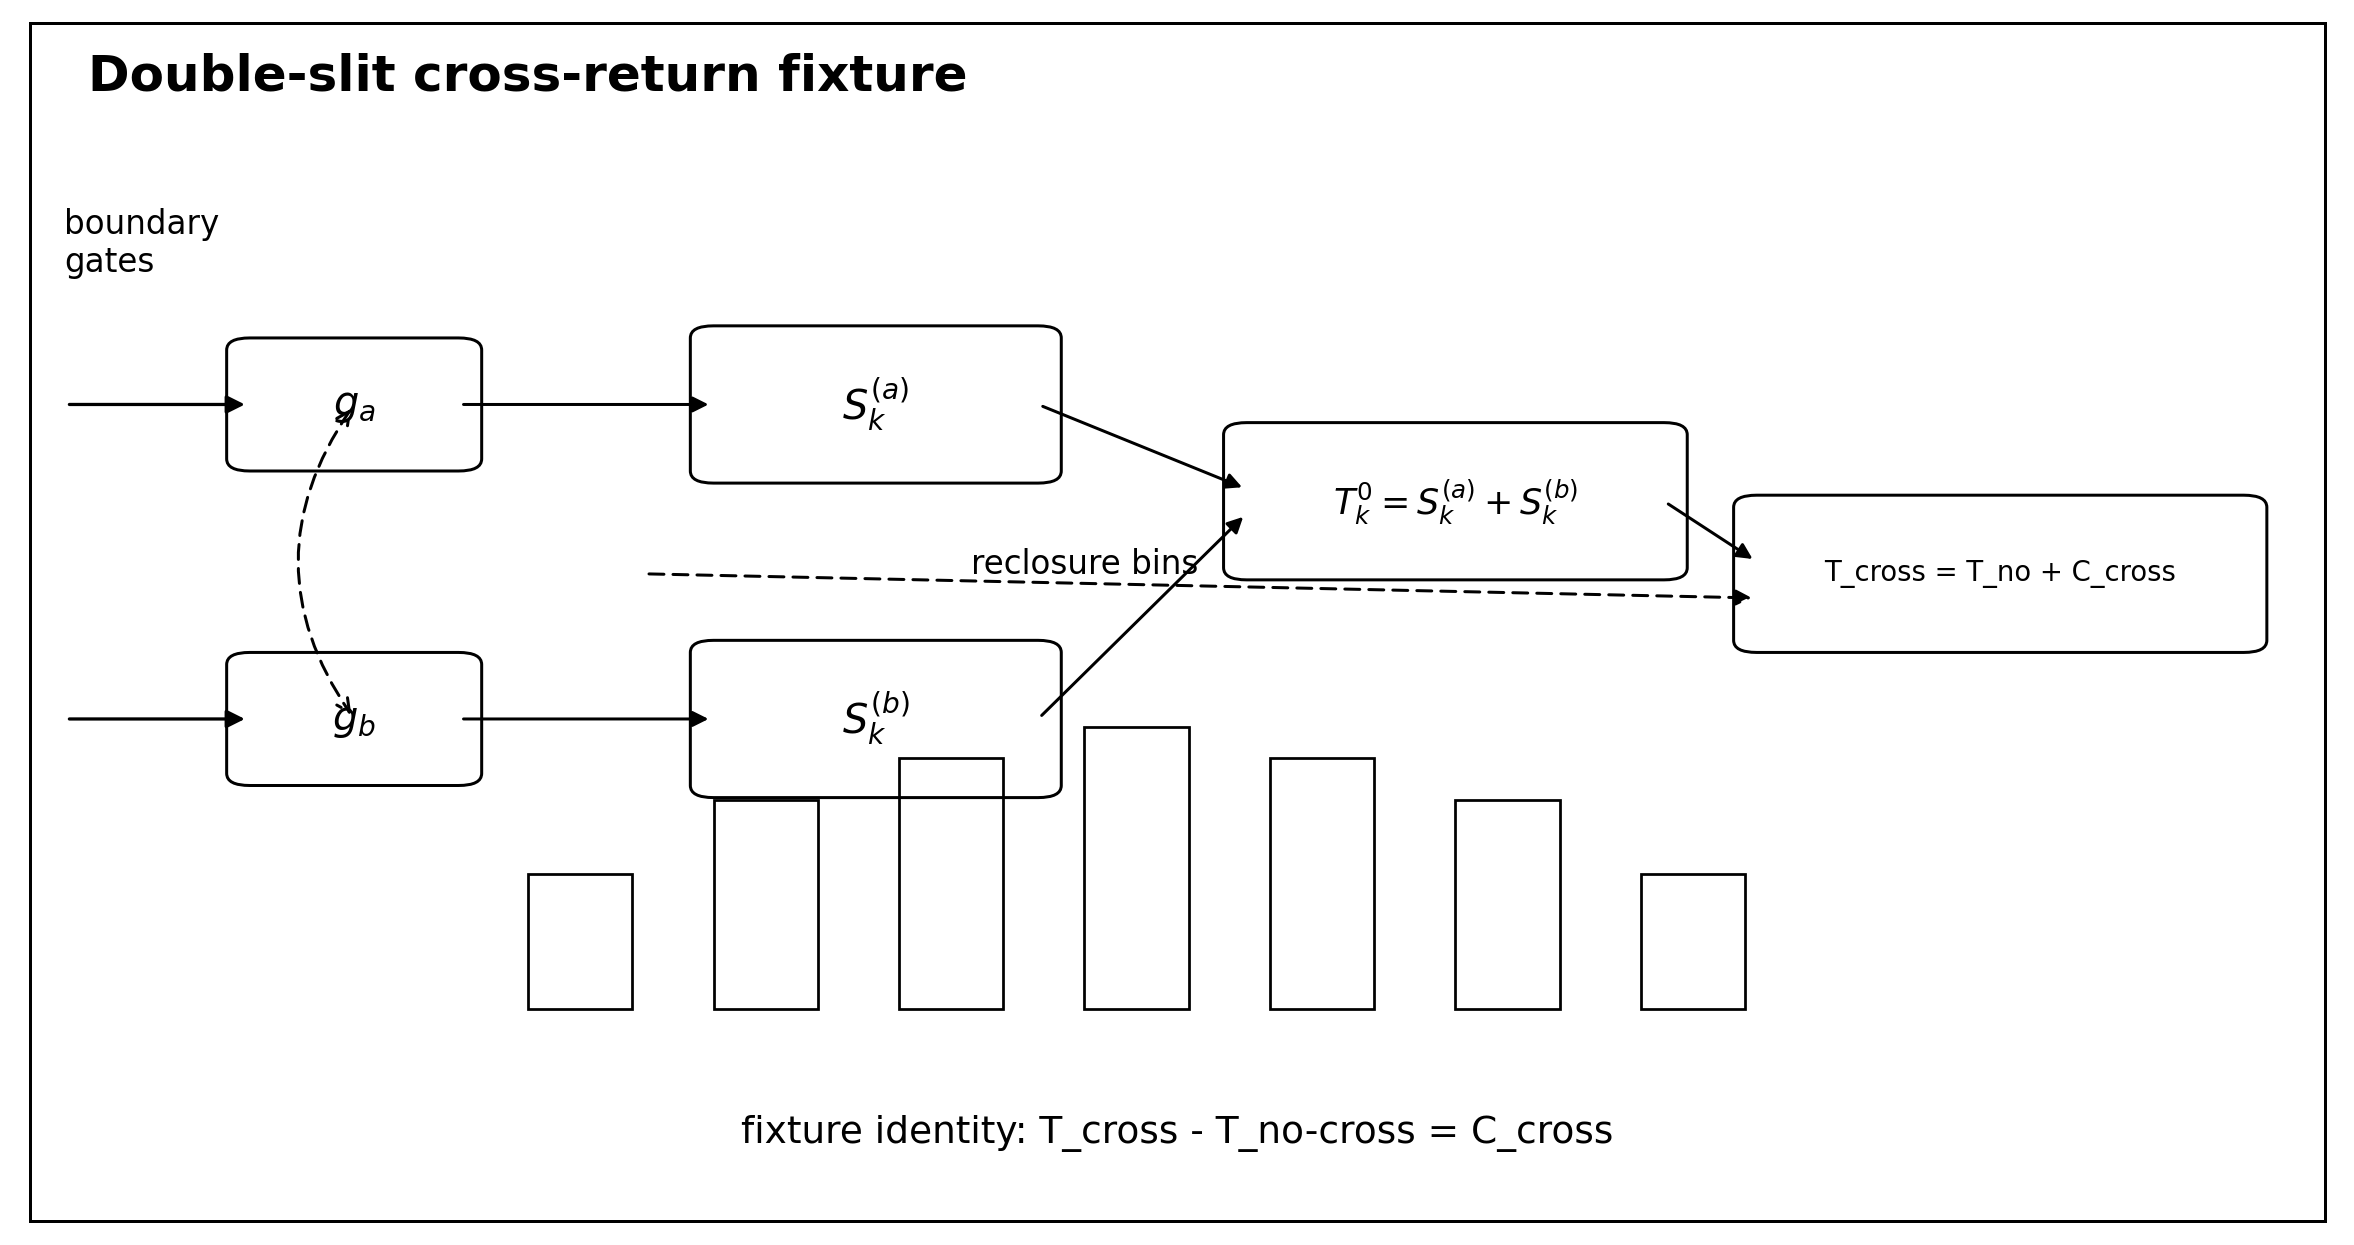
\includegraphics[width=0.95\textwidth]{figures/double_slit_cross_return_setup.png}
\caption{Recurrent-ring double-slit cross-return setup. Two boundary gates produce independent one-gate contributions; the no-cross baseline is the sum of one-gate contributions, and the cross-return contribution produces the declared cross-return fixture.}
\label{fig:manual-recurrent-ring-double-slit}
\end{figure}

The independent two-gate baseline is
\[
T^0_k=S^{(a)}_k+S^{(b)}_k.
\]
The cross-return contribution is
\[
C^\times_k(B)=C_{ab,k}^{\times}(B)
=
\sum_{t\in\omega}
\sum_{\gamma:g_a\leftrightarrow g_b\leadsto k}
\kappa_k\SADARop_{B|t}(C_\gamma).
\]
The recurrent ring value is
\[
T^\times_k=T^0_k+C^\times_k.
\]
Thus the audit identity is
\[
\boxed{
T^\times_k-T^0_k=C^\times_k.
}
\]


\subsubsection{Exact double-slit fixture}\label{manual:cross-return:exact-double-slit-fixture}
The following fixture is a released A\(\Omega\)-internal exact integer bin test. The independent gate-sum value is \(T_k^0\). The recurrent ring value is \(T_k^\times\). The declared fixture comparator is \(O_k\). The comparison is the exact \(\delta_3\) tally \(\delta_{3,k}(T^\times,O)=(s_k^{(3)},m_k)\).

\begin{table}[h]
\centering
\scriptsize
\caption{Dimonhexon slit handoff: exact \(\delta_3\) reclosure-bin fixture.}
\begin{tabular}{r r r r r r r r}
\toprule
$k$ & $S_k$ & $T^0_k$ & $C^\times_k$ & $T^\times_k$ & $O_k$ & $\Delta^{\mathbb Z}_k$ & $\delta_{3,k}$\\
\midrule
$-5$ & 4 & 8 & 0 & 8 & 8 & 0 & $(0,0)$\\
$-4$ & 9 & 18 & -8 & 10 & 11 & -1 & $(-1,1)$\\
$-3$ & 16 & 32 & -12 & 20 & 19 & 1 & $(+1,1)$\\
$-2$ & 25 & 50 & 8 & 58 & 59 & -1 & $(-1,1)$\\
$-1$ & 31 & 62 & 18 & 80 & 79 & 1 & $(+1,1)$\\
$0$ & 35 & 70 & 26 & 96 & 95 & 1 & $(+1,1)$\\
$1$ & 31 & 62 & 18 & 80 & 80 & 0 & $(0,0)$\\
$2$ & 25 & 50 & 8 & 58 & 58 & 0 & $(0,0)$\\
$3$ & 16 & 32 & -12 & 20 & 21 & -1 & $(-1,1)$\\
$4$ & 9 & 18 & -8 & 10 & 10 & 0 & $(0,0)$\\
$5$ & 4 & 8 & 0 & 8 & 8 & 0 & $(0,0)$\\
\bottomrule
\end{tabular}
\label{tab:manual-dimonhexon-double-slit-fixture}
\end{table}

Here \(C^\times_k=T^\times_k-T^0_k\). The center-bin fixture is
\[
T^\times_0=96,
\qquad
O_0=95,
\qquad
\Delta^{\mathbb Z}_0=1,
\qquad
\delta_{3,0}=(+1,1).
\]
The full-fixture checks are
\[
\sum_kT_k^\times=448,
\qquad
\sum_kO_k=448,
\qquad
\sum_k\Delta^{\mathbb Z}_k=0,
\qquad
\sum_km_k=6.
\]

\begin{figure}[h]
\centering
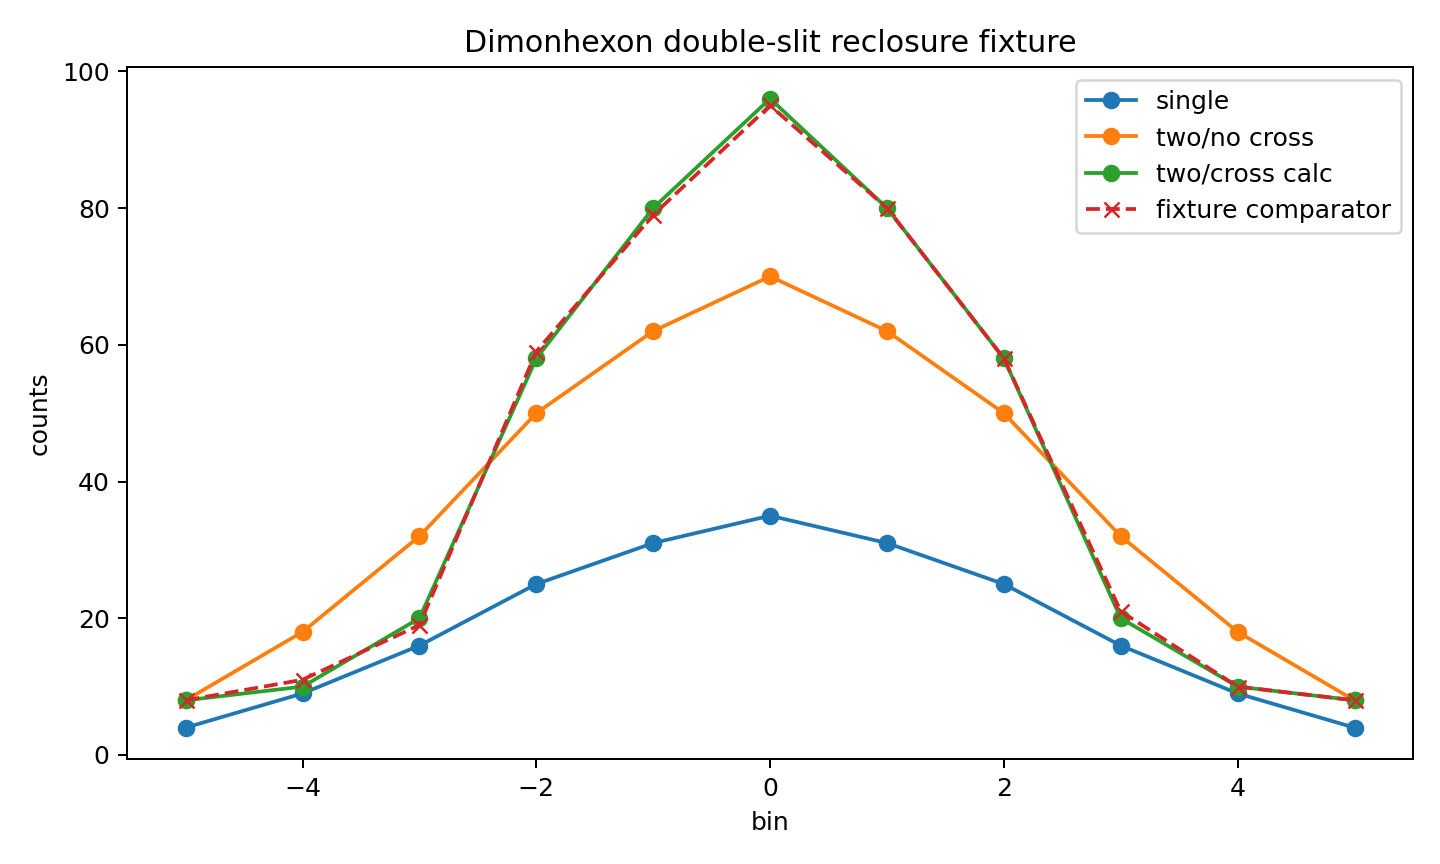
\includegraphics[width=0.82\textwidth]{figures/double_slit_reclosure_fixture.png}
\caption{Dimonhexon double-slit reclosure fixture. Cross-return changes the two-gate distribution; the exact internal comparison is recorded by \(\delta_3\).}
\label{fig:manual-double-slit-reclosure-fixture}
\end{figure}

\begin{table}[h]
\centering
\scriptsize
\caption{Recurrent-ring cross-return symbol table.}
\begin{tabular}{l l}
\toprule
Symbol & Meaning\\
\midrule
$S^{(a)}_k$ & one-gate contribution from $g_a$ into bin $k$\\
$S^{(b)}_k$ & one-gate contribution from $g_b$ into bin $k$\\
$T^0_k$ & independent gate-sum value\\
$C_{ab,k}^{\times}(B)$ & cross-return contribution from $g_a\leftrightarrow g_b$ into bin $k$\\
$T^\times_k$ & recurrent ring value\\
$O_k$ & declared fixture comparator, if used\\
$\Delta_k^{\mathbb Z}$ & exact signed integer fixture residual\\
$\delta_{3,k}(T^\times,O)$ & exact ternary signed residual tally\\
\bottomrule
\end{tabular}
\label{tab:manual-recurrent-ring-symbols}
\end{table}

\aodnoteblock{Status}{Released A\(\leftrightarrow\Omega\)-internal field-ring fixture.}
\aodprovenance{main:subsec:fractal-field-ring-gate; main:eq:b-scoped-flux; main:eq:frg-cross-return-contribution; manual \secref{manual:cross-return:dimonhexon-slit}.}
\aodremark{The independent gate-sum value records independent reclosure. The recurrent ring value records redistributed returned-current coupling.}

\subsection{Short-window fixture scope}\label{manual:short-window:scope}
\aodnoteblock{Scope}{This section is A\(\Omega\)-internal. It tests short-window \(\rho^D\)-clipping, pending overhang, closure residual, and sheddic path status without external comparison.}

Declare the short-window fixture scope
\[
\mathbf a_{\mathrm{sw}}\vdash(F_{\mathrm{sw}},R_{\mathrm{sw}},\partial R_{\mathrm{sw}},\omega_{\mathrm{sw}}),
\qquad
B_{\mathrm{sw}}=(\partial F_{\mathrm{sw}},\omega_{\mathrm{sw}}).
\]
The baseline Dimonon support used below is
\[
\Pi(1{:}2)=2^1+2=4,
\qquad
H_\mu=1,
\qquad
\rho^D_{1{:}2}=RD^{(1)}(1{:}2)=2\cdot4+1=9.
\]
The record length is denoted by \(L_M\). It is distinct from the path-derived scalar \(\rho^D\).

\begin{figure}[h]
\centering
\scriptsize
\begin{tikzpicture}[node distance=0.55cm, every node/.style={rounded corners, draw, align=center, inner sep=4pt}]
\node (scope) {short-window scope\\$B_{\mathrm{sw}}=(\partial F_{\mathrm{sw}},\omega_{\mathrm{sw}})$};
\node[below=of scope] (rd) {path support\\$\rho^D=RD^{(1)}(1{:}2)=9$};
\node[below=of rd] (clip) {clip\\$\rho^D_\omega=\min(\rho^D,|\omega|)$};
\node[below left=0.65cm and 1.2cm of clip] (overhang) {pending overhang\\$Q^D=C_3\max(0,\rho^D-|\omega|)$};
\node[below right=0.65cm and 1.2cm of clip] (closure) {closure residual\\$\Delta^{\mathrm{close}}=P^D-C^{\mathrm{close}}$};
\node[below=1.0cm of clip] (shed) {shedding\\$X_{\mathrm{shedding}}=\max(0,\Delta^{\mathrm{close}})$};
\draw[-{Latex}] (scope) -- (rd);
\draw[-{Latex}] (rd) -- (clip);
\draw[-{Latex}] (clip) -- (overhang);
\draw[-{Latex}] (clip) -- (closure);
\draw[-{Latex}] (closure) -- (shed);
\end{tikzpicture}
\caption{Short-window RCD fixture flow. The path-derived \(\rho^D\) is clipped by the declared window to produce \(\rho^D_\omega\), while pending overhang \(Q^D\) and closure residual \(\Delta^{\mathrm{close}}\) are kept separate from shedding excess.}
\label{fig:manual-short-window-setup}
\end{figure}

\subsection{Shared fixture equations}\label{manual:short-window:equations}
For a candidate record \(M\) in a declared scope \(B\), use
\[
\rho^D_\omega(M;B)=\min(\rho^D(M;B),|\omega|),
\]
\[
Q^D(M;B)
=
C_3\max(0,\rho^D(M;B)-|\omega|),
\]
\[
P^D(M;B)=C_3\rho^D_\omega(M;B),
\]
\[
\Delta^{\mathrm{close}}(M;B)=P^D(M;B)-C^{\mathrm{close}}(M;B),
\]
\[
X_{\mathrm{shedding}}(M;B)=\max(0,\Delta^{\mathrm{close}}(M;B)).
\]
\aodnoteblock{Remark}{\(\Delta^{\mathrm{close}}\) records signed closure residual. \(X_{\mathrm{shedding}}\) records only positive surplus. Negative closure residuals are retained as deficits or open checks, not as sheddic surplus.}

\subsection{Closure-dependent and surplus fixtures}\label{manual:short-window:fixture-table}
The following table keeps \(\Delta^{\mathrm{close}}\) and \(X_{\mathrm{shedding}}\) separate. This prevents closure-deficit records from being misread as sheddic surplus.

\begin{table}[h]
\centering
\scriptsize
\caption{Short-window RCD and shedding fixtures. All records use \(C_3=3\) and \(\rho^D=RD^{(1)}(1{:}2)=9\).}
\begin{tabular}{c c c c c c c c c c}
\toprule
Row & \(C_3\) & \(\rho^D\) & \(L_M\) & \(|\omega|\) & \(\rho^D_\omega\) & \(Q^D\) & \(P^D\) & \(C^{\mathrm{close}}\) & \(\Delta^{\mathrm{close}},X_{\mathrm{shedding}}\)\\
\midrule
\(1{:}2{:}7\to C_6\) & 3 & 9 & 7 & 7 & 7 & 6 & 21 & 18 & \(3,3\)\\
\(1{:}2{:}7\to C_8\) & 3 & 9 & 7 & 7 & 7 & 6 & 21 & 24 & \(-3,0\)\\
\(1{:}2{:}9\to C_8\) & 3 & 9 & 9 & 9 & 9 & 0 & 27 & 24 & \(3,3\)\\
\(1{:}2{:}10\to C_{10}\) & 3 & 9 & 10 & 10 & 9 & 0 & 27 & 27 & \(0,0\)\\
\bottomrule
\end{tabular}
\label{tab:manual-short-window-fixtures}
\end{table}

\subsection{The \texorpdfstring{\(1{:}2{:}7\)}{1:2:7} closure-dependent fixture}\label{manual:short-window:127}
For \(1{:}2{:}7\), the window is shorter than the path-derived support:
\[
\rho^D_\omega=\min(9,7)=7,
\qquad
Q^D=3(9-7)=6,
\qquad
P^D=3\cdot7=21.
\]
Against lower closure \(C_6=18\), the fixture carries surplus:
\[
\Delta^{\mathrm{close}}=21-18=3,
\qquad
X_{\mathrm{shedding}}=3.
\]
Against upper closure \(C_8=24\), the fixture is closure-deficient:
\[
\Delta^{\mathrm{close}}=21-24=-3,
\qquad
X_{\mathrm{shedding}}=0.
\]
Thus \(1{:}2{:}7\) is closure-dependent.

\subsection{The \texorpdfstring{\(1{:}2{:}9\)}{1:2:9} surplus fixture}\label{manual:short-window:129}
For \(1{:}2{:}9\), the candidate window reaches the path-derived support:
\[
\rho^D_\omega=\min(9,9)=9,
\qquad
Q^D=0,
\qquad
P^D=3\cdot9=27.
\]
Against the \(C_8=24\) closure record,
\[
\Delta^{\mathrm{close}}=27-24=3,
\qquad
X_{\mathrm{shedding}}=3.
\]
This is the nine-window surplus fixture.

\subsection{The \texorpdfstring{\(1{:}2{:}10\)}{1:2:10} clipped retained fixture}\label{manual:short-window:1210}
For \(1{:}2{:}10\), the candidate record length exceeds the path-derived support:
\[
\rho^D_\omega=\min(9,10)=9,
\qquad
Q^D=0,
\qquad
P^D=27.
\]
Against \(C_{10}=27\),
\[
\Delta^{\mathrm{close}}=0,
\qquad
X_{\mathrm{shedding}}=0.
\]
The fixture is a clipped retained check.

\subsection{Sheddic path audit}\label{manual:short-window:shedpath-audit}
The sheddic path audit uses
\[
\mathrm{SheddicPath}(X_{\mathrm{shedding}})
\in
\{E_2,\mathsf C_6,\mathsf C_8,\mathsf C_{10},\ldots,\mathsf C_{2n}\}.
\]
A surplus fixture must declare where the positive \(X_{\mathrm{shedding}}\) is routed. A deficit fixture may remain an open check or may be paired with a declared closure completion.

\subsection{Audit hooks}\label{manual:short-window:audit-hooks}
\aodnoteblock{Audit}{A short-window fixture records \(\rho^D_\omega\), \(Q^D\), \(\Delta^{\mathrm{close}}\), and \(X_{\mathrm{shedding}}\) separately. Sheddic surplus is positive only, and every positive \(X_{\mathrm{shedding}}\) carries a declared sheddic path.}
\aodprovenance{main:eq:window-clipped-rho; main:eq:burden-overhang; main:eq:sheddic-path; manual \secref{manual:short-window:scope}.}
\aodremark{This section is A\(\Omega\)-internal. It prepares the mechanics used by rest-energy records and boundary-current records without adding an external comparison target.}
